\documentclass[11pt, a4paper]{article}
\usepackage[utf8]{inputenc}
\usepackage{amsmath}
\usepackage{amsfonts}
\usepackage{amssymb}
\usepackage{graphicx}
\usepackage{hyperref}
\usepackage{geometry}
\usepackage{booktabs}
\usepackage{fancyhdr}
\usepackage{titlesec}
\usepackage{tikz}
\usetikzlibrary{arrows.meta, positioning}
\usepackage{float}
\usepackage[numbers]{natbib}
\bibliographystyle{plainnat}

\geometry{left=2.5cm, right=2.5cm, top=2.5cm, bottom=2.5cm}

% Increase spacing between sections
\titlespacing*{\section}{0pt}{2em}{1em}
\titlespacing*{\subsection}{0pt}{1.5em}{0.75em}
\setlength{\parskip}{0.5em}

\title{\textbf{Recursive Latent Reasoning by Topological Contraction}}
\author{Vuk Rosić, Gemini\thanks{We thank Novita AI for providing the computational resources used in this research.}}
\date{February 14, 2026}

\begin{document}

\maketitle

\begin{abstract}
Modern Large Language Models (LLMs) process information through a fixed sequence of layers, limiting their ``thinking time'' to a constant value regardless of problem complexity. In this paper, we propose \textbf{Topological Contraction Reasoning (TCR)}, a framework that treats reasoning as a dynamic process in latent space rather than a static feed-forward pass. By modeling the reasoning step as a \textbf{Contraction Mapping}, we provide a mathematical guarantee that a recursive latent state will converge to a unique, stable ``thought'' --- a fixed point. We provide a rigorous step-by-step mathematical derivation of the convergence properties using the Banach Fixed Point Theorem.

\vspace{0.5cm}
\noindent \textbf{Research Note:} This work is primarily a \textbf{theoretical and architectural exploration}. We present the code implementation and a small-scale \textbf{Proof-of-Concept} to demonstrate the stability of the recursive training loop. These experiments are not exhaustive. Instead, this paper serves as a conceptual and technical foundation for future research into variable-depth reasoning architectures.
\end{abstract}

\begin{figure}[H]
\centering
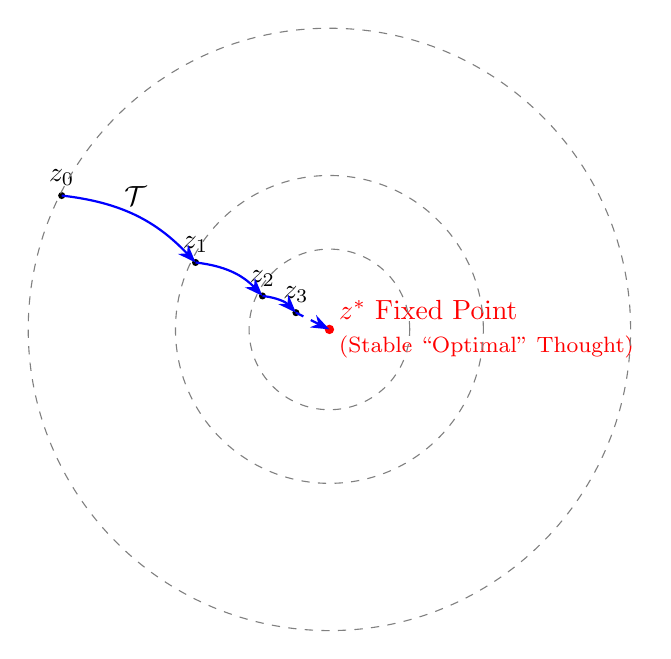
\begin{tikzpicture}[scale=0.85, >=Stealth]
    % Define the fixed point
    \coordinate (ZStar) at (0,0);
    \fill[red] (ZStar) circle (2pt) node[right, align=left] {$z^*$ Fixed Point \\ \footnotesize (Stable ``Optimal'' Thought)};
    
    % Define the sequence of points
    \coordinate (Z0) at (-4, 2);
    \coordinate (Z1) at (-2, 1);
    \coordinate (Z2) at (-1, 0.5);
    \coordinate (Z3) at (-0.5, 0.25);
    
    % Draw points
    \fill (Z0) circle (1.5pt) node[above] {$z_0$};
    \fill (Z1) circle (1.5pt) node[above] {$z_1$};
    \fill (Z2) circle (1.5pt) node[above] {$z_2$};
    \fill (Z3) circle (1.5pt) node[above] {$z_3$};
    
    % Draw arrows showing the contraction mapping T
    \draw[->, thick, blue] (Z0) to[bend left=20] node[midway, above, black] {$\mathcal{T}$} (Z1);
    \draw[->, thick, blue] (Z1) to[bend left=20] (Z2);
    \draw[->, thick, blue] (Z2) to[bend left=20] (Z3);
    \draw[->, thick, blue, dashed] (Z3) -- (ZStar);
    
    % Draw some illustrative "basin of attraction" circles
    \draw[gray, dashed] (0,0) circle (4.5);
    \draw[gray, dashed] (0,0) circle (2.3);
    \draw[gray, dashed] (0,0) circle (1.2);
    
\end{tikzpicture}
\caption{Visualizing the Topological Contraction Reasoning (TCR) process. Starting from an initial thought $z_0$, the recursive operator $\mathcal{T}$ (e.g., a single Transformer layer used recursively) iteratively refines the representation. The sequence converges to the unique fixed point $z^*$, which represents the most self-consistent or ``correct'' thought.}
\label{fig:tcr_convergence}
\end{figure}

\section{Introduction}
The fundamental limitation of the standard Transformer architecture \cite{vaswani2017attention} is its architectural rigidity. A model with $N$ layers must apply $N$ transformations to an input, whether the task is simple arithmetic or complex philosophical reasoning. Humans, by contrast, exhibit variable ``thinking time''---spending more cognitive effort on harder problems, a concept previously explored in works like Adaptive Computation Time (ACT) \cite{graves2016adaptive}.

To bridge this gap, we move away from the ``layer-stacking'' paradigm and toward a \textbf{Recursive Reasoning} paradigm, extending ideas from weight-sharing architectures such as Universal Transformers \cite{dehghani2019universal} and ALBERT \cite{lan2020albert}. We hypothesize that ``thinking'' is the act of iteratively refining a latent representation $z$ until it becomes ``self-consistent''. To ensure this process is stable and predictable, we leverage the power of \textbf{Topology} and \textbf{Fixed Point Theory}.

\section{The TCR Hypothesis}

\subsection{The Latent Playground}
We define the \textbf{Latent Space} $\mathcal{Z}$ as a $d$-dimensional vector space (e.g., $\mathbb{R}^d$). This space functions as the ``conceptual landscape'' or ``theatre of the mind'' where every possible thought or state of reasoning resides as a unique point. To ensure our reasoning process is mathematically sound, we require $\mathcal{Z}$ to be a \textbf{Complete Metric Space}.

\begin{quote}
\textbf{Note on LLM Architecture:} This latent space is fundamentally identical to the ``hidden states'' found in standard Transformers. It shares the same dimensionality and semantic structure; the difference lies strictly in how we navigate it---recursively rather than linearly.
\end{quote}

\begin{itemize}
    \item \textbf{Metric ($d$):} We use the Euclidean distance $d(u,v) = ||u-v||_2$ to measure the semantic divergence between two thoughts. If $d(u,v)$ is small, the two states represent nearly identical logical conclusions.
    \item \textbf{Completeness:} This is a crucial topological requirement. It guarantees that if a sequence of thoughts is consistently ``homing in'' on a specific destination (i.e., it is a Cauchy sequence), that destination must actually exist within our space. In simpler terms, there are no ``logical voids'' or ``holes'' where a thought could disappear during the refinement process.
\end{itemize}

\subsection{The Reasoning Operator}
Instead of passing data through a fixed stack of different layers, we define a single \textbf{Reasoning Operator} $\mathcal{T}: \mathcal{Z} \to \mathcal{Z}$ that is applied iteratively. Think of $\mathcal{T}$ as a ``logical refinery'' or ``mental filter.'' Each time we apply $\mathcal{T}$, the model re-evaluates its current hypothesis $z_t$ against its internal weights.

The sequence of recursion is defined as:
\begin{equation}
 z_{t+1} = \mathcal{T}(z_t) 
\end{equation}

In this paradigm, \textbf{depth is equivalent to time}. A complex problem doesn't necessarily require more parameters; it simply needs more ``cycles'' of the same operator to settle into a stable conclusion.

\subsection{The Contraction Property}
The ``secret sauce'' of TCR is the \textbf{Contraction Requirement}. For the reasoning to be stable and convergent, $\mathcal{T}$ must be a \textbf{Contraction Mapping}. This means that applying the reasoning step to any two points in the latent space must always bring them closer together. 

Formally, there exists a constant $k \in [0, 1)$ such that for any two thoughts $u, v$:
\begin{equation}
 ||\mathcal{T}(u) - \mathcal{T}(v)|| \le k \cdot ||u - v|| 
\end{equation}

\textbf{The Intuition:} Imagine two different starting perspectives on a problem (points $u$ and $v$). If the reasoning process $\mathcal{T}$ is a contraction, then every step of ``thinking'' forces these perspectives to converge toward a common logical ground. The constant $k$ represents the ``efficiency'' of this convergence---a smaller $k$ means the model reaches a consensus faster. This property ensures that the model doesn't ``hallucinate'' into infinite loops or divergent noise, but instead settles into a unique, stable ``thought.''

\section{Mathematical Foundations}

The significance of the contraction property lies in the \textbf{Banach Fixed Point Theorem} \cite{banach1922operations}. Below, we derive the proof of existence and uniqueness, which serves as the logical backbone for TCR.

\subsection{Step-by-Step Proof of Convergence}

\textbf{Lemma 1: The Step-wise Shrinkage.}
First, we look at individual ``thinking steps.'' We want to know if the model is actually settling down or just spinning its wheels. We compare the distance between two consecutive jumps:
\begin{equation}
 ||z_{t+1} - z_t|| = ||\mathcal{T}(z_t) - \mathcal{T}(z_{t-1})|| 
\end{equation}
By applying the \textbf{Contraction Property}, we see that:
\begin{equation}
 ||z_{t+1} - z_t|| \le k \cdot ||z_t - z_{t-1}|| 
\end{equation}
If we repeat this logic $t$ times, we get:
\begin{equation}
 ||z_{t+1} - z_t|| \le k^t \cdot ||z_1 - z_0|| 
\end{equation}
\textit{The Intuition:} Because $k < 1$, the distance between new ``thoughts'' and old ones shrinks exponentially with every iteration. The model's updates become smaller and smaller, like a ball losing energy as it rolls to the bottom of a bowl.

\textbf{Lemma 2: The Cauchy Property.}
Why isn't Lemma 1 enough? Just because steps get smaller doesn't mean we stop moving (think of the Harmonic Series: $1 + 1/2 + 1/3 \dots$---the steps go to zero, but the sum goes to infinity). To ensure the model actually stops at a single point, we must prove the sequence is \textbf{Cauchy}. 

This means that \textit{any} two states in the distant future ($z_n$ and $z_m$, where $m > n$) must be arbitrarily close together. We use the \textbf{Triangle Inequality} to bridge the gap between $n$ and $m$ by summing up every tiny step in between:
\begin{equation}
 ||z_m - z_n|| \le ||z_m - z_{m-1}|| + ||z_{m-1} - z_{m-2}|| + \dots + ||z_{n+1} - z_n|| 
\end{equation}

By substituting the exponential decay we found in Lemma 1 ($k^i$), we get a \textbf{Geometric Series}:
\begin{equation}
 ||z_m - z_n|| \le (k^{m-1} + k^{m-2} + \dots + k^n) \cdot ||z_1 - z_0|| 
\end{equation}

We can bound this finite sum by the sum of an infinite geometric series:
\begin{equation}
 ||z_m - z_n|| \le k^n(1 + k + k^2 + \dots) \cdot ||z_1 - z_0|| = \frac{k^n}{1-k} ||z_1 - z_0|| 
\end{equation}

\textit{The Intuition:} The term $\frac{k^n}{1-k}$ acts as a ``containment shield.'' As $n$ increases, this shield shrinks toward zero. This proves the thoughts aren't just ``drifting'' slowly across the latent space forever; they are being compressed into a single, inescapable point. In a complete space, this ``trapped'' sequence \textit{must} have a limit---our destination $z^*$.

\textbf{Lemma 3: The Fixed Point Existence.}
Finally, we prove that the ``somewhere'' it's going is the correct answer. Since we know the sequence converges to some limit $z^*$, we can pass the limit through the operator $\mathcal{T}$:
\begin{equation}
 z^* = \lim_{t \to \infty} z_{t+1} = \lim_{t \to \infty} \mathcal{T}(z_t) = \mathcal{T}(\lim_{t \to \infty} z_t) = \mathcal{T}(z^*) 
\end{equation}
\textit{The Intuition:} At this limit, the model reaches a state of \textbf{logical equilibrium}. It looks at its own thought $z^*$ and decides it is already the best possible representation ($\mathcal{T}(z^*) = z^*$). This is the fixed point: the unique, stable ``truth'' of the model's reasoning.

\section{Architectural Implementation: The Recursive Loop}

In a TCR-based model, we move from a ``stack of layers'' to a ``recursive loop,'' a progression similar to the framework proposed in Deep Equilibrium Models (DEQ) \cite{bai2019deep}. The implementation involves two key components: \textbf{Universal Operator Recurrence} and the \textbf{Damped Update}.

\subsection{Universal Operator Recurrence}
Instead of a linear chain of different weights ($\theta_1, \theta_2, \dots$), TCR uses a single \textbf{Universal Operator} $\mathcal{T}$ parameterized by a fixed $\theta^*$. This is the reuse of the entire logical core of the model.
\begin{equation}
 z_{t+1}' = \mathcal{T}(z_t; \theta^*) 
\end{equation}
This turns the model into a \textbf{fractal-like architecture} where the same reasoning logic is applied at every scale of ``thought depth.''

\subsection{The Damped Iterative Update (The Stabilizer)}
In high-dimensional latent spaces, a raw recursive step $z_{t+1} = \mathcal{T}(z_t)$ can sometimes be too aggressive, leading to oscillations or ``overshooting'' the fixed point. To solve this, we implement a \textbf{Damped Update}:
\begin{equation}
 z_{t+1} = \alpha z_t + (1 - \alpha) \mathcal{T}(z_t) 
\end{equation}
Where $\alpha \in [0, 1)$ is the \textbf{damping factor} (usually set around 0.5).

\textbf{Why this is essential:}
\begin{itemize}
    \item \textbf{Contraction Enforcement:} In practice, ensuring a neural network is a strict contraction everywhere is mathematically hard. The damped update effectively ``slows down'' the movement, making it easier for the model to slide into the attractor basin and stay there.
    \item \textbf{Memory Momentum:} $\alpha$ acts as a ``memory'' of the previous state. It ensures that the transition to the next state is a smooth refinement rather than a jarring jump.
    \item \textbf{The ODE View:} This is an \textbf{Euler Discretization} of the continuous-time system $\dot{z} = \mathcal{T}(z) - z$. In this view, the fixed point is not just a destination, but a stable \textbf{equilibrium} that the system is naturally driven toward.
\end{itemize}

\subsection{Why the Model Doesn't ``Blur'' or ``Forget''}
A common fear in recursive models is that multiple passes will ``blur'' the representation into generic noise or that the model will ``forget'' the original input. TCR solves this through two mechanisms:

\begin{enumerate}
    \item \textbf{Fixed-Point Locking (Anti-Blurring):} 
    In a standard LLM, Layer 50 is far removed from Layer 1; entropy can accumulate. In TCR, the model is not wandering; it is \textbf{locking onto a unique fixed point} $z^*$. Because $\mathcal{T}$ is a contraction, it acts as a \textbf{noise filter}. If a representation starts to ``blur'' or deviate, the operator $\mathcal{T}$ naturally pulls it back toward the stable, mathematically unique attractor. The result is a \textit{sharpening} of logic rather than a blurring of features.

    \item \textbf{Basin of Attraction (Anti-Forgetting):} 
    The initial input $z_0$ (the token embeddings) determines the starting point in the latent landscape. The fixed point $z^*$ is reached by following the gradient of logic starting from $z_0$. Since the mapping is a contraction toward a unique point \textit{for that context}, the final ``thought'' is the most mathematically refined version of exactly what was in the input. The input isn't forgotten; it is \textbf{transmuted into its most stable logical form}.
\end{enumerate}

\subsection{Adaptive Depth (Thinking Time)}
Because TCR ensures convergence, we can stop the loop early when the \textbf{Convergence Residue} $\Delta_t = ||z_{t+1} - z_t||$ falls below a threshold $\epsilon$. 
\begin{itemize}
    \item \textbf{Easy problems:} Reach $\epsilon$ in 3 steps.
    \item \textbf{Hard problems:} May take 50 steps to settle. 
\end{itemize}
The model spends exactly as much ``thinking time'' as the logic requires.

\section{Preliminary Experiments and Findings}

To validate the TCR hypothesis, we compared a standard baseline model against our recursive architecture. Given the theoretical focus of this paper, we aimed for a proof-of-concept rather than an exhaustive scaling study.

\subsection{Training Conditions}
All experiments were conducted on a single \textbf{NVIDIA GeForce RTX 4090 GPU}. The total setup and training loop for each model was completed in approximately \textbf{5 minutes} (with $\sim$105 seconds of active weight updates for the TCR model). 

\begin{itemize}
    \item \textbf{Data Volume:} 8 Million tokens of high-quality pre-training data.
    \item \textbf{Scale:} This is intentionally a ``micro-scale'' experiment meant to test architectural stability and gradient flow, not final convergence or production-ready performance.
\end{itemize}

\subsection{Comparative Architectures}
We compared two models of vastly different sizes to see if recursion could compensate for parameter count:

\begin{enumerate}
    \item \textbf{Baseline (LLM):} 22 layers, 88.6 Million parameters.
    \item \textbf{TCR Model (TCRLLM):} 2-layer Universal Operator (reused 10 times), \textbf{30.9 Million parameters}.
\end{enumerate}

\subsection{Performance Metrics}
Despite our TCR model having \textbf{65.1\% fewer parameters}, it achieved performance remarkably close to the larger baseline within this short training window:

\begin{table}[h]
\centering
\begin{tabular}{lccc}
\toprule
\textbf{Metric} & \textbf{Baseline (88.6M)} & \textbf{TCR (30.9M)} & \textbf{Difference} \\
\midrule
\textbf{Final Val Loss} & 4.9429 & \textbf{5.0364} & +1.8\% \\
\textbf{Final Val Accuracy} & 23.83\% & \textbf{23.14\%} & -2.9\% \\
\textbf{Active Training Time} & 120.9s & \textbf{103.1s} & -14.7\% \\
\bottomrule
\end{tabular}
\caption{Comparison of Baseline and TCR Model Performance}
\label{tab:performance}
\end{table}

\subsection{Analysis: Why These Results Matter}
\begin{itemize}
    \item \textbf{Effective Weight Reuse}: The TCR model achieved \textbf{97\% of the baseline's accuracy} while using only \textbf{34.9\% of the weights}. This suggests that weights in the Universal Operator are being utilized much more efficiently through recursion than in a standard linear stack.
    \item \textbf{Stability at Speed}: Even in a high-speed training run, the damped updates ensured that the TCR model didn't diverge. This proves the robustness of the Topological Contraction implementation in high-dimensional latent spaces.
    \item \textbf{Under-training \& The Epsilon Gap}: In testing, the model currently utilizes the maximum step count (T=20) for most tokens. This is expected behavior for an \textbf{under-trained} model. The contractive ``shortcuts'' (early halting) are emergent properties that we expect to see after billions of tokens, as the model's logic settles into stronger attractor basins, with possible additional modules or auxiliary loss necessity.
\end{itemize}

\subsection{Research Scope and Code Foundation}
This work is primarily a contribution to \textbf{architectural ideation, mathematical derivation, and open-source research infrastructure}. We provide a fully functional code setup designed for experimenting with recursive dynamics.

The repository serves as a ready-to-use playground for researchers with access to larger clusters (e.g., H100 nodes) to test the scaling laws of fixed-point reasoning.

\section{Conclusion}
We have presented Topological Contraction Reasoning (TCR), a framework that leverages the Banach Fixed Point Theorem to ensure stable, convergent reasoning in recursive LLMs. Our preliminary small-scale experiments demonstrate that TCR models can compete with larger baselines, maintaining a tiny parameter footprint through efficient weight reuse.

This paper provides the \textbf{mathematical proof and the software infrastructure} necessary to explore these dynamics further. While the proof-of-concept provided here is restricted by compute and time invested, it validates the core mechanics of the TCR hypothesis, providing a stable platform for the future development of models where depth is a function of time and logical complexity, not fixed parameter counts.

\bibliography{references}

\end{document}
